%%%%%%%%%%%%%%%%%%%%%%%%%%%%%%%%%%%%%%%%%
% Short Sectioned Assignment LaTeX Template Version 1.0 (5/5/12)
% This template has been downloaded from: http://www.LaTeXTemplates.com
% Original author:  Frits Wenneker (http://www.howtotex.com)
% License: CC BY-NC-SA 3.0 (http://creativecommons.org/licenses/by-nc-sa/3.0/)
%%%%%%%%%%%%%%%%%%%%%%%%%%%%%%%%%%%%%%%%%

%----------------------------------------------------------------------------------------
%	PACKAGES AND OTHER DOCUMENT CONFIGURATIONS
%----------------------------------------------------------------------------------------

\documentclass[paper=a4, fontsize=11pt]{scrartcl} % A4 paper and 11pt font size

% ---- Entrada y salida de texto -----

\usepackage[T1]{fontenc} % Use 8-bit encoding that has 256 glyphs
\usepackage[utf8]{inputenc}
%\usepackage{fourier} % Use the Adobe Utopia font for the document - comment this line to return to the LaTeX default

% ---- Idioma --------

\usepackage[spanish, es-tabla]{babel} % Selecciona el español para palabras introducidas automáticamente, p.ej. "septiembre" en la fecha y especifica que se use la palabra Tabla en vez de Cuadro

% ---- Otros paquetes ----

\usepackage{url} % ,href} %para incluir URLs e hipervínculos dentro del texto (aunque hay que instalar href)
\usepackage{amsmath,amsfonts,amsthm} % Math packages
%\usepackage{graphics,graphicx, floatrow} %para incluir imágenes y notas en las imágenes
\usepackage{graphics,graphicx, float, subfig} %para incluir imágenes y colocarlas

% Para hacer tablas comlejas
%\usepackage{multirow}
%\usepackage{threeparttable}

%\usepackage{sectsty} % Allows customizing section commands
%\allsectionsfont{\centering \normalfont\scshape} % Make all sections centered, the default font and small caps

\usepackage{fancyhdr} % Custom headers and footers
\pagestyle{fancyplain} % Makes all pages in the document conform to the custom headers and footers
\usepackage{eurosym} % Para poder añadir el símbolo del euro
\fancyhead{} % No page header - if you want one, create it in the same way as the footers below
\fancyfoot[L]{} % Empty left footer
\fancyfoot[C]{} % Empty center footer
\fancyfoot[R]{\thepage} % Page numbering for right footer
\renewcommand{\headrulewidth}{0pt} % Remove header underlines
\renewcommand{\footrulewidth}{0pt} % Remove footer underlines
\setlength{\headheight}{13.6pt} % Customize the height of the header

\numberwithin{equation}{section} % Number equations within sections (i.e. 1.1, 1.2, 2.1, 2.2 instead of 1, 2, 3, 4)
\numberwithin{figure}{section} % Number figures within sections (i.e. 1.1, 1.2, 2.1, 2.2 instead of 1, 2, 3, 4)
\numberwithin{table}{section} % Number tables within sections (i.e. 1.1, 1.2, 2.1, 2.2 instead of 1, 2, 3, 4)

\setlength\parindent{0pt} % Removes all indentation from paragraphs - comment this line for an assignment with lots of text

\newcommand{\horrule}[1]{\rule{\linewidth}{#1}} % Create horizontal rule command with 1 argument of height

\usepackage{listings}
\usepackage{dsfont}
\usepackage{booktabs}
%----------------------------------------------------------------------------------------
%	TÍTULO Y DATOS DEL ALUMNO
%----------------------------------------------------------------------------------------

\title{	
\normalfont \normalsize 
\textsc{\textbf{Taller de Geometría y Topología} \\ Grado en Matemáticas \\ Universidad de Granada} \\ [25pt] % Your university, school and/or department name(s)
\horrule{0.5pt} \\[0.4cm] % Thin top horizontal rule
\huge Ejercicios del Grupo 3  \\ % The assignment title
Universos
\horrule{2pt} \\[0.5cm] % Thick bottom horizontal rule
}
\author{	
		Elena Tudela Castro \\
		Raimundo Morales Solier \\
		Simón López Vico \\
		Francisco Leopoldo Gallego Salido \\
		Alberto Jesús Durán López} % Nombre y apellidos
\date{\normalsize\today} % Incluye la fecha actual

%----------------------------------------------------------------------------------------
% DOCUMENTO
%----------------------------------------------------------------------------------------

\begin{document}

\maketitle % Muestra el Título

\newpage %inserta un salto de página

%\tableofcontents % para generar el índice de contenidos

% \listoffigures

% \listoftables



\section{Universo}

\textbf{Página 8}

\begin{enumerate}
\item Como seres de dimensión 3 en un mundo de tres dimensiones es fácil dibujar y entender posibles formas de Planilandia pero no de nuestro propio Universo. Imaginar la forma de nuestro Universo en alguna de las siguientes situaciones:

	\begin{itemize}
	\item Hacemos una expedición a una galaxia remota. Al llegar a ella descubrimos estar de vuelta en la tierra.
	
	Un toro o un cilindro en dimensión 3.
	
	\item Un astrónomo acaba de descubrir que los mismos objetos se encuentran en posiciones distintas del Universo.
	
	Entendiendo que posición distinta se refiere a con forma invertida, puede tener forma de una botella de Klein o una cinta de Möbius en dimensión 3.
	
	\item Buscando ondas de radio que detecten señales extraterrestres, detectamos una señal que procede de una galaxia lejana. Investigamos y vemos que se trata de la señal de un programa de TV emitido hace 50 años.
	
	Ya que las señales de radio van en todas direcciones, podrían venir de cualquier parte, por lo que debería de tener forma de toro. Aparte, al captar las ondas de tan solo 50 años atrás, podemos suponer que el toro es muy pequeño.
	
	\end{itemize}
\end{enumerate}

\textbf{Páginas 10, 12 y 13}
\begin{enumerate}
\item ¿Cuáles de las siguientes superficies tienen la misma topología?

\begin{figure}[H]
\centering
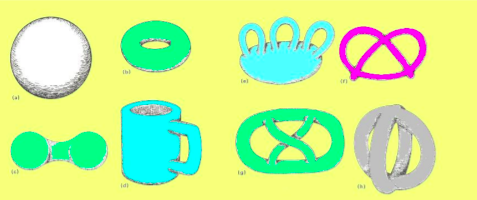
\includegraphics[scale=0.5]{images/universo/pagina_10_1.png}
\end{figure}
Tendrán la misma topología a y c (esfera); b y d (toro); e, f, g y h (3-toro).

\item En Planilandia CP descubrió que dos caminos cerrados partiendo del mismo punto en direcciones opuestas no tienen por qué volver a cruzarse en un punto diferente. ¿Es esta propiedad geométrica o topológica?

Independientemente de la deformación realizada sobre la superficie, los dos
caminos cerrados no se cruzarán (ni antes ni ahora), y por tanto la propiedad permanece inalterable aunque deformemos la superficie deduciendo así que es una propiedad topológica.

\item Describir superficies con la misma topología pero diferente geometría?

Las figuras que hemos visto en el ejercicio 1 con misma topología tienen distinta geometría, pues la curvatura difiere en diversos puntos. Además, simplemente realizando una homotecia sobre una superficie, su geometría cambia, pues se modifica su curvatura.

\item Distingue según su topología intrínseca y extrínseca:

\begin{figure}[H]
\centering
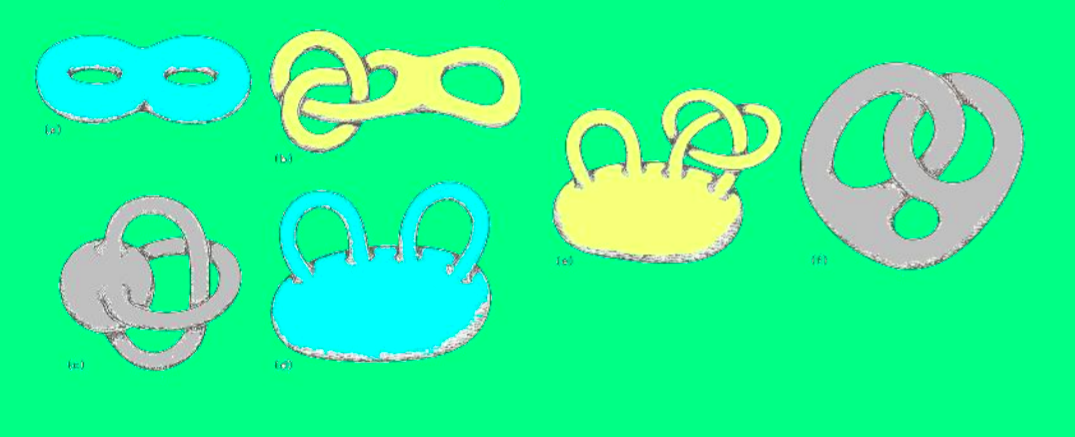
\includegraphics[scale=0.25]{images/universo/pagina_12_1.png}
\end{figure}

Todas tienen la misma topología intrínseca, pues representan un 2-toro.

Misma topología extrínseca: (a, c d, f) y (b,e)

\item ¿Puedes forrar un cilindro con parte de una hoja de papel sin deformarla? ¿Y un cono? ¿Y un trozo de esfera?

\begin{itemize}

\item Cilindro con bases no se puede. Sin bases sí se puede

\item Un cono viene dado por $\{(x,y,x) \in \mathbb{R}^{3}  : x^2 + y^2 = z^2\} $
 
Si tomamos el cono con $z\leq0$ ó $z\geq0$ sí se puede. Con ambas partes no.
\item En una esfera tampoco.

\end{itemize}

\item ¿Cómo pueden los planilandés que vivan en mundos como los de la figura conocer que sus geometrías intrínsecas son diferentes? ¿Qué pueden decir acerca de sus topologías extrínsecas e intrínsecas?

Construyendo un triángulo lo suficientemente grande, si están en un plano la suma de sus ángulos será $\pi$; en una geometría esférica la suma será mayor que $\pi$; y en una geometría hiperbólica, menor que $\pi$.

\end{enumerate}

\textbf{Páginas 20, 21 y 24}

\begin{enumerate}
\item En el siguiente tablero de ajedrez sobre un toro llano, ¿qué figuras están amenazadas por el caballo blanco?

Marcamos las figuras amenazadas en rojo.

\begin{figure}[H]
\centering
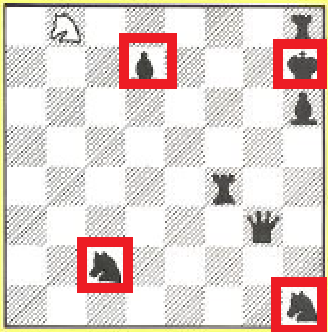
\includegraphics[scale=0.75]{images/universo/pagina_20_1_sol.png}
\end{figure}

\item ¿Qué figuras están amenazadas por el caballo y la reina blancos?

Están amenazadas todas las figuras.
\begin{figure}[H]
\centering
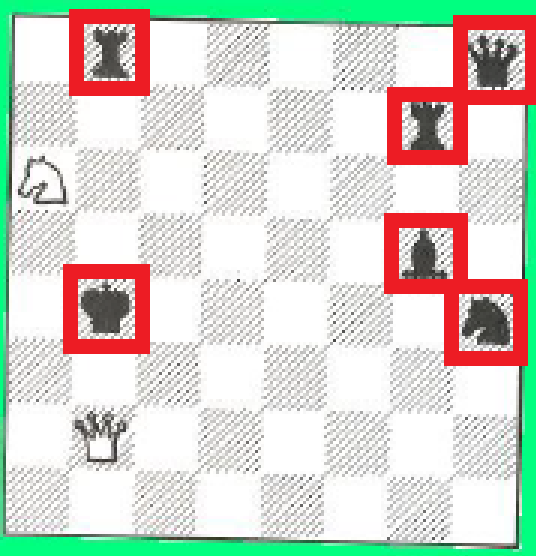
\includegraphics[scale=0.45]{images/universo/pagina_21_1_sol.png}
\end{figure}

\item Las siguientes figuras muestran un toro llano de tres dimensiones. Explica cómo se construye e imagina que verías al mirar en una dirección concreta.

\begin{figure}[H]
\centering
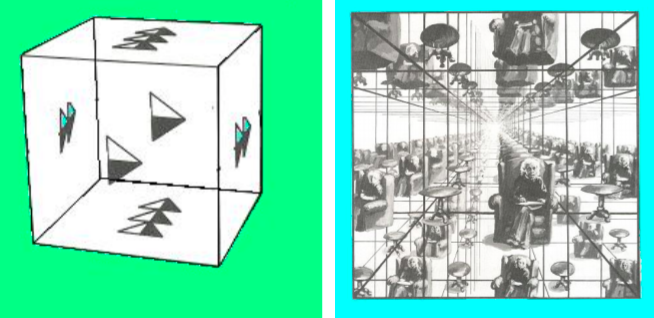
\includegraphics[scale=0.35]{images/universo/pagina_21_2.png}
\end{figure}

Se construye identificando las caras opuestas. Al mirar hacia arriba veríamos nuestros pies, al mirar hacia delante veríamos nuestra espalda, al mirar hacia la izquierda, veríamos nuestro perfil derecho, etc. En definitiva, veríamos el lado opuesto de nuestro cuerpo a la dirección de nuestra mirada.

\item ¿Cuáles de las siguientes posiciones ganan en el juego de tres en raya dentro de una botella de Klein?

\begin{figure}[H]
\centering
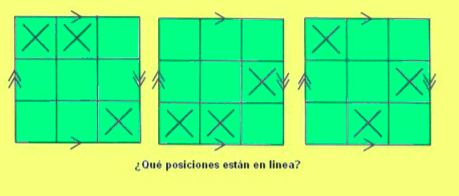
\includegraphics[scale=0.5]{images/universo/pagina_24_1.png}
\end{figure}

Las tres posiciones ganan el juego dentro de una botella de Klein.

\item Analiza como hacer tres en linea en la siguiente figura:

Marcamos la X en el tablero con la que se ganará el juego en una botella de Klein.

\begin{figure}[H]
\centering
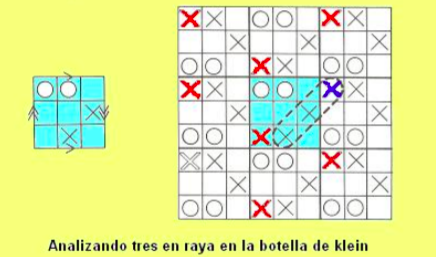
\includegraphics[scale=0.35]{images/universo/pagina_24_2.png}
\end{figure}

\begin{figure}[H]
	\centering
	\subfloat[]{
		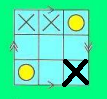
\includegraphics[scale=0.79]{images/universo/pagina_24_2_a.png}
		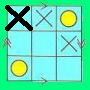
\includegraphics[scale=0.85]{images/universo/pagina_24_2_b.png}
		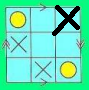
\includegraphics[scale=0.848]{images/universo/pagina_24_2_c.png}
		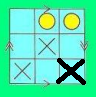
\includegraphics[scale=0.8]{images/universo/pagina_24_2_d.png}
		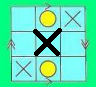
\includegraphics[scale=0.88]{images/universo/pagina_24_2_e.png}
	}
\end{figure}


\end{enumerate}

\textbf{Página 30}
\begin{enumerate}
\item Si un planilandés viviendo en un plano proyectivo cruza el ecuador, ¿vuelve como su imagen especular?

Sí, ya que el plano proyectivo identifica los puntos de los bordes con la misma dirección, de manera que aparecería de forma invertida.

\item Una familia de planilandeses vive en un plano proyectivo. Planean edificar dos gasolineras separadas cuanto más mejor. ¿Dónde deberían construirlas?

Se deberían construir una en el polo Norte o Sur y otra en cualquier punto del ecuador.

\item CP conoce que vive en una esfera o en un plano proyectivo. ¿Cómo podría saber cuál de los dos es su mundo?

Dando una vuelta completa al mundo; si CP vuelve a la posición inicial de forma inversa, estará en un plano proyectivo.

\item Un segundo planilandés sabe que su Universo es un plano proyectivo o una botella de Klein, ¿qué podría hacer para conocer de cual de los dos se trata?

Este planilandés deberá dar dos vueltas a su mundo, una en una dirección inicial elegida y otra perpendicularmente a ésta, desde una posición inicial. Si en ambas vuelve de forma inversa estará en un plano proyectivo. Si únicamente se invierte una vez de las dos vueltas dadas, estará en una botella de Klein.

\end{enumerate}

\textbf{Página 37}

\begin{enumerate}
\item Deducir que si a una cinta de Mobius le pegamos un disco por el borde obtenemos un plano proyectivo.

\begin{figure}[H]
\centering
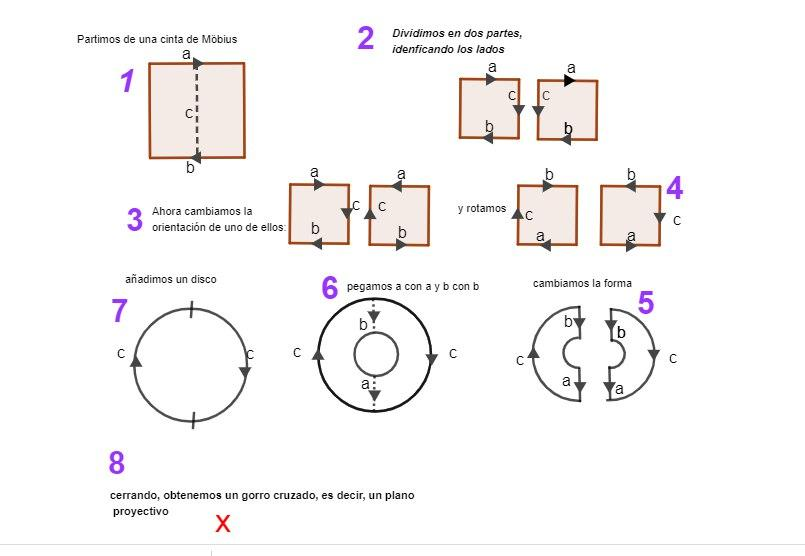
\includegraphics[scale=0.6]{images/universo/pagina_37_1.jpg}
\end{figure}

\item Corrobora las palabras de Klein: "La cinta de Mobius es divina, si pegas dos por su borde obtiene mi botella"

La cinta de Möbius es igual a un plano proyectivo al que le hemos quitado un disco.

La botella de Klein es igual a la suma conexa de dos planos proyectivos.

La suma conexa consiste en tomar dos superficies, quitarle un disco a cada una y unirlas por los bordes formados en la superficie.

Por tanto, para formar una botella de Klein, tomamos dos planos proyectivos y le quitamos un disco a cada uno de ellos para realizar la suma conexa, obteniendo así dos cintas de Möbius que al pegar por su borde obtenemos la botella de Klein.

\item Construye usando papel la suma conexa de una cinta de Mobius a un toro y a una botella de Klein.

Lo construimos con Geogebra. Empecemos por la cinta de Mobius y el toro.

\begin{figure}[H]
\centering
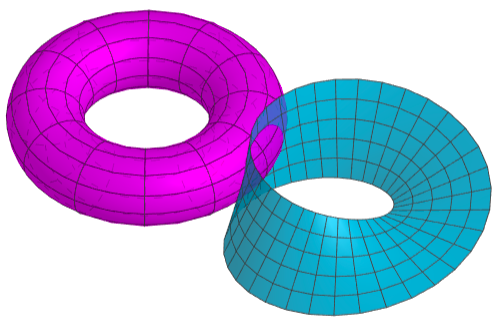
\includegraphics[scale=0.4]{images/universo/toro_mobius_1.png}
\end{figure}

En la imagen superior, hemos de imaginar que en la intersección de las dos superficies no hay nada, y que la parte rosa del toro que sobresale en la cinta de Mobius no está. Por tanto, estaremos poniendo una cinta de Mobius sin un disco, que es un plano proyectivo como hemos visto anteriormente, en un agujero de un toro, obteniendo un toro con un gorro cruzado.

\begin{figure}[H]
\centering
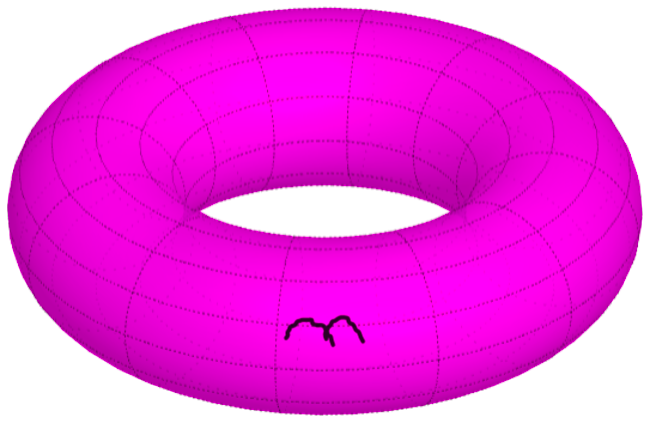
\includegraphics[scale=0.25]{images/universo/toro_mobius_2.png}
\end{figure}

Dibujar la botella de Klein en Geogebra es bastante complicado, pero podemos deducir que la suma conexa de un proyectivo con una botella es topológicamente equivalente, como podemos ver en éste\footnote{\url{https://www.youtube.com/watch?v=aBbDvKq4JqE}} vídeo; además, reincidiremos con cuestiones teóricas este hecho en el siguiente ejercicio.

\begin{figure}[H]
\centering
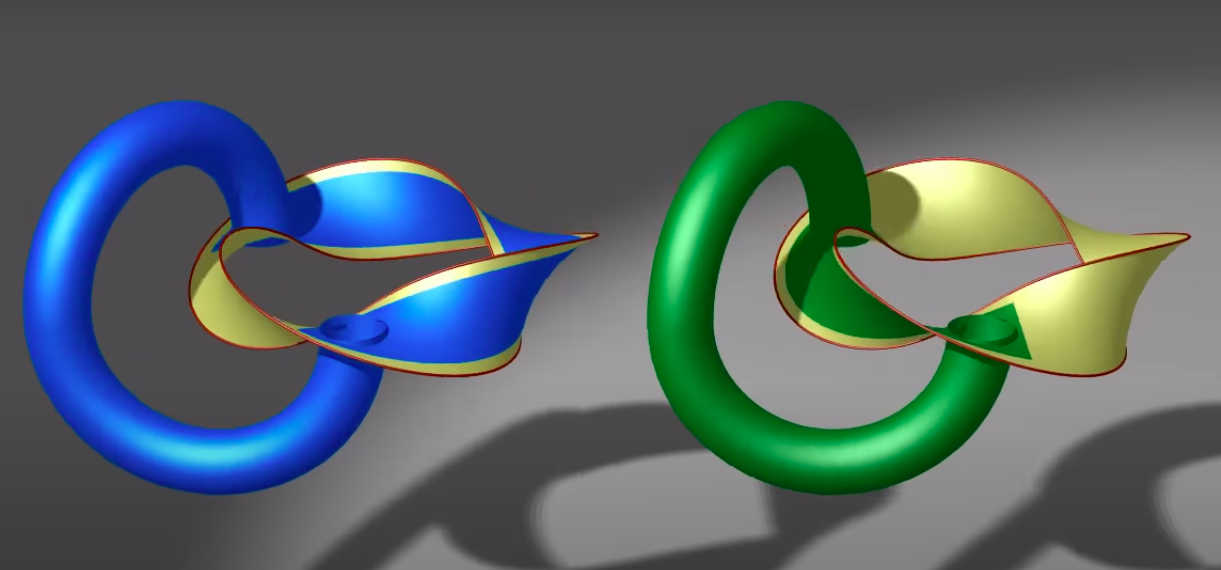
\includegraphics[scale=0.25]{images/universo/torus_klein_mobius.png}
\end{figure}

\item Muestra que la suma conexa de un toro con un plano proyectivo es topológicamente equivalente a la suma conexa de una botella de Klein con un plano proyectivo.

Sabemos por la teoría que un toro junto a un plano proyectivo es topológicamente equivalente a tres planos proyectivos (una esfera con un asa y un gorro cruzado es igual a tres gorros cruzados), y también sabemos que dos planos proyectivos son topológicamente equivalentes a una botella de Klein. Por tanto, la suma de un toro con un proyectivo son tres proyectivos, que es topológicamente equivalente a un proyectivo y una botella de Klein.

\item Establece una correspondencia por equivalencia topológica entre las superficies de los conjuntos A y B.

\begin{figure}[H]
\centering
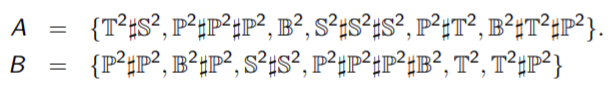
\includegraphics[scale=0.5]{images/universo/pagina_37_1.png}
\end{figure}

\begin{itemize}
\item $\mathds{T}^2\#\mathds{S}^2 \equiv \mathds{T}^2$
\item $\mathds{P}^2\#\mathds{P}^2\#\mathds{P}^2 \equiv \mathds{B}^2\#\mathds{P}^2$
\item $\mathds{B}^2 \equiv \mathds{P}^2\#\mathds{P}^2$
\item $\mathds{S}^2\#\mathds{S}^2\#\mathds{S}^2 \equiv \mathds{S}^2\#\mathds{S}^2$
\item $\mathds{P}^2\#\mathds{T}^2 \equiv \mathds{T}^2\#\mathds{P}^2$
\item $\mathds{B}^2\#\mathds{T}^2\#\mathds{P}^2 \equiv \mathds{P}^2\#\mathds{P}^2\#\mathds{P}^2\#\mathds{B}^2$
\end{itemize}

\end{enumerate}

\vspace{0.6cm}

\textbf{Descripción de al menos 4 universos tridimensionales finitos.}

\begin{enumerate}
\item Toro llano de 3 dimensiones:

Sería un espacio generado por un cubo repetido a lo largo de los ejes. Este cubo tendría las caras opuestas identificadas como indicamos en la siguiente imagen. 

\begin{figure}[H]
	\centering
	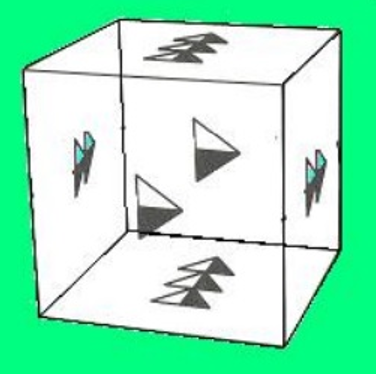
\includegraphics[scale=0.5]{images/universo/universo_1_1.png}
\end{figure}


De esta forma si nos situamos en el centro del cubo al mirar al frente veríamos nuestra espalda, si miramos hacia arriba veríamos nuestros pies, mirando hacia abajo veríamos nuestra cabeza y mirando uno de los lados veríamos nuestro lado opuesto al que miramos. Esto se puede entender más fácilmente observando la siguiente imagen.

\begin{figure}[H]
	\centering
	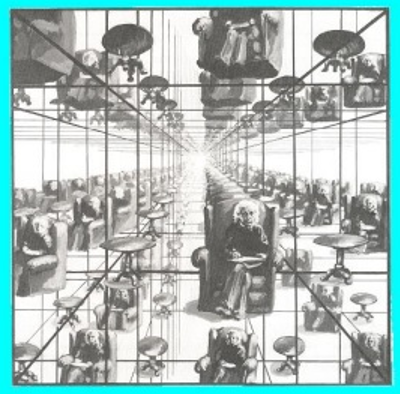
\includegraphics[scale=0.5]{images/universo/universo_1_2.png}
\end{figure}


Es fácil comprobar que de esta forma con el cubo rellenamos todo R3 .


\item Otra identificación del cubo en 3 dimensiones:

Sería un espacio parecido al anterior ya que su “dominio fundamental” está formada también por un cubo, pero esta vez con un cubo que tendría las siguientes identificaciones 

\begin{figure}[H]
	\centering
	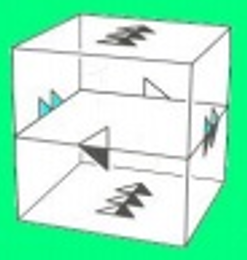
\includegraphics[scale=0.7]{images/universo/universo_2_1.png}
\end{figure}


De esta forma vemos que podríamos decir que una de las caras está identificada de forma “inversa”. En este caso si miramos hacia arriba o hacia uno de los lados sucedería lo mismo que en el toro, pero no es así en el caso de mirar hacia delante o hacia atrás. En este caso debemos de distinguir que al estar identificadas de esta manera si entramos por la parte de la derecha de una de las caras saldremos a la misma altura por la parte de la izquierda de la cara opuesta y viceversa en el caso de entrar por la parte de la izquierda de una de las caras. Entonces al rellenar todo R3 si nos situásemos en el centro del cubo nos veríamos a nosotros como en el Toro llano de 3 dimensiones, pero con la parte de la derecha en la izquierda y la de la izquierda en la derecha. 



\item  Botella de Klein de 3 dimensiones:

Volvemos a un espacio generado por un cubo en el cual identificamos las caras como se muestra en la siguiente imagen 

\begin{figure}[H]
	\centering
	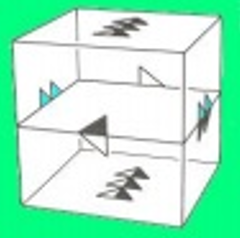
\includegraphics[scale=0.7]{images/universo/universo_3_1.png}
\end{figure}

Con estas identificaciones volvemos al caso de antes, pero con una variación más, y es que cuando entramos por la cara delantera (o trasera) a parte de salir por la contraria invirtiendo izquierda y derecha también saldríamos baca abajo, es decir, lo que está arriba pasaría a estar abajo y lo que está abajo pasaría a estar arriba. La siguiente imagen puede ayudarnos a verlo más fácilmente 

\begin{figure}[H]
	\centering
	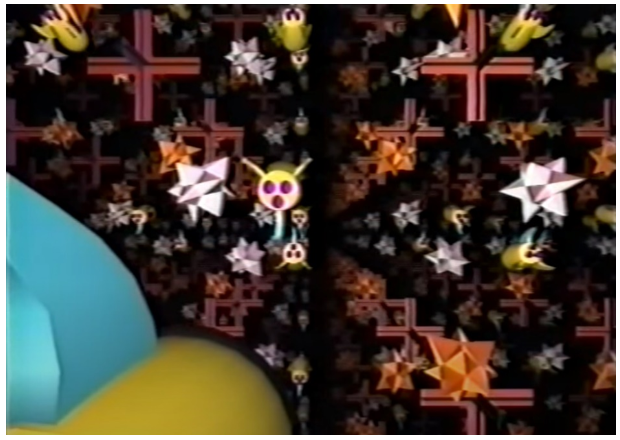
\includegraphics[scale=0.5]{images/universo/universo_3_2.png}
\end{figure}
\end{enumerate}






\newpage
\begin{thebibliography}{X}

\bibitem{1} \textsc{Apuntes de Clase}

\end{thebibliography}


\end{document}

